\section{Node Class Reference}
\label{classNode}\index{Node@{Node}}
{\tt \#include $<$node.h$>$}

Inheritance diagram for Node::\begin{figure}[H]
\begin{center}
\leavevmode
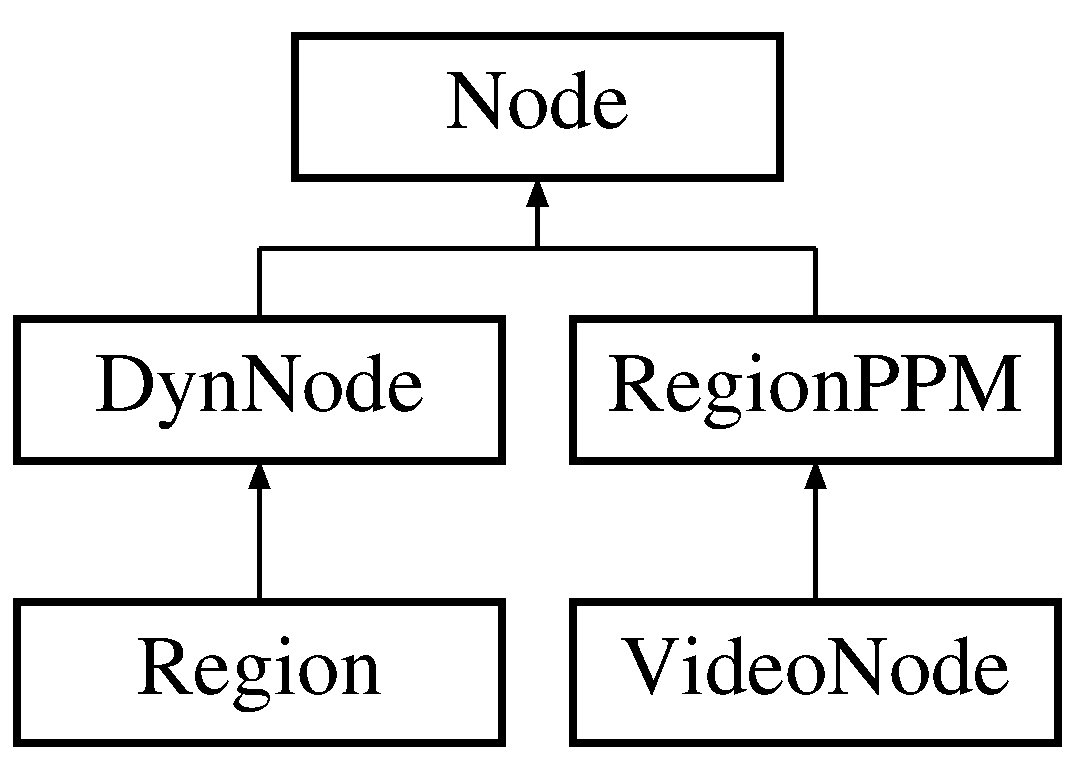
\includegraphics[height=3cm]{classNode}
\end{center}
\end{figure}
\subsection*{Public Member Functions}
\begin{CompactItemize}
\item 
int {\bf getColor} () const
\item 
void {\bf setColor} (int \_\-col)
\item 
{\bf Node} ()
\item 
void {\bf setNodeNumVar} (int \_\-n)
\item 
void {\bf setNodeId} (string \_\-s)
\item 
void {\bf setBelief} ({\bf Belief} $\ast$b)
\item 
{\bf Node} (string s, int {\bf numVar}, {\bf Belief} $\ast$bp=0, int \_\-type=-1)
\item 
int {\bf getNodeNumVar} () const
\item 
string {\bf getNodeId} () const
\item 
{\bf Belief} $\ast$ {\bf getBeliefPtr} ()
\item 
{\bf $\sim$Node} ()
\end{CompactItemize}
\subsection*{Private Attributes}
\begin{CompactItemize}
\item 
int {\bf numVar}
\begin{CompactList}\small\item\em the number of variables at this node \item\end{CompactList}\item 
string {\bf id}
\begin{CompactList}\small\item\em the unique string identifier for this node \item\end{CompactList}\item 
{\bf Belief} $\ast$ {\bf bPtr}
\begin{CompactList}\small\item\em set of beliefs about current state \item\end{CompactList}\item 
{\bf NodeType} {\bf type}
\begin{CompactList}\small\item\em the type of node \item\end{CompactList}\item 
int {\bf color}
\begin{CompactList}\small\item\em used in graph algorithms \item\end{CompactList}\end{CompactItemize}
\subsection*{Friends}
\begin{CompactItemize}
\item 
ostream \& {\bf operator$<$$<$} (ostream \&os, {\bf Node} \&n)
\end{CompactItemize}


\subsection{Detailed Description}
The node class has the following convention regarding naming of the nodes Variable nodes are named as VXXXX ( where XXXX represent numeric code) for example, V012 Factor nodes are named as F\_\-VXXX\_\-VXX ( F representing its a factor ) and VXXX represent the 



\subsection{Constructor \& Destructor Documentation}
\index{Node@{Node}!Node@{Node}}
\index{Node@{Node}!Node@{Node}}
\subsubsection{\setlength{\rightskip}{0pt plus 5cm}Node::Node ()\hspace{0.3cm}{\tt  [inline]}}\label{classNode_74f89688a500bb12a891b0c521284ae1}


\index{Node@{Node}!Node@{Node}}
\index{Node@{Node}!Node@{Node}}
\subsubsection{\setlength{\rightskip}{0pt plus 5cm}Node::Node (string {\em s}, int {\em numVar}, {\bf Belief} $\ast$ {\em bp} = {\tt 0}, int {\em \_\-type} = {\tt -1})}\label{classNode_4ad7f425f80a8769a08aa91f2aa4a542}


\index{Node@{Node}!~Node@{$\sim$Node}}
\index{~Node@{$\sim$Node}!Node@{Node}}
\subsubsection{\setlength{\rightskip}{0pt plus 5cm}Node::$\sim$Node ()\hspace{0.3cm}{\tt  [inline]}}\label{classNode_261e6a1e75de946e7feacb3007165435}




\subsection{Member Function Documentation}
\index{Node@{Node}!getColor@{getColor}}
\index{getColor@{getColor}!Node@{Node}}
\subsubsection{\setlength{\rightskip}{0pt plus 5cm}int Node::getColor () const\hspace{0.3cm}{\tt  [inline]}}\label{classNode_1abe470a6d6918e996c11392cc9c0c20}


\index{Node@{Node}!setColor@{setColor}}
\index{setColor@{setColor}!Node@{Node}}
\subsubsection{\setlength{\rightskip}{0pt plus 5cm}void Node::setColor (int {\em \_\-col})\hspace{0.3cm}{\tt  [inline]}}\label{classNode_85dad9bdc7f7f9564fe432099567b2a6}


\index{Node@{Node}!setNodeNumVar@{setNodeNumVar}}
\index{setNodeNumVar@{setNodeNumVar}!Node@{Node}}
\subsubsection{\setlength{\rightskip}{0pt plus 5cm}void Node::setNodeNumVar (int {\em \_\-n})\hspace{0.3cm}{\tt  [inline]}}\label{classNode_e5c45d621acfbee49dd0b70d10ca3f87}


\index{Node@{Node}!setNodeId@{setNodeId}}
\index{setNodeId@{setNodeId}!Node@{Node}}
\subsubsection{\setlength{\rightskip}{0pt plus 5cm}void Node::setNodeId (string {\em \_\-s})\hspace{0.3cm}{\tt  [inline]}}\label{classNode_9352e0f15cc3ddae82082a59be82d5c2}


\index{Node@{Node}!setBelief@{setBelief}}
\index{setBelief@{setBelief}!Node@{Node}}
\subsubsection{\setlength{\rightskip}{0pt plus 5cm}void Node::setBelief ({\bf Belief} $\ast$ {\em b})\hspace{0.3cm}{\tt  [inline]}}\label{classNode_04293dd9093d19f40f71b2dd67472a59}


\index{Node@{Node}!getNodeNumVar@{getNodeNumVar}}
\index{getNodeNumVar@{getNodeNumVar}!Node@{Node}}
\subsubsection{\setlength{\rightskip}{0pt plus 5cm}int Node::getNodeNumVar () const\hspace{0.3cm}{\tt  [inline]}}\label{classNode_8502fcc64beead4af76420747a22c8ed}


\index{Node@{Node}!getNodeId@{getNodeId}}
\index{getNodeId@{getNodeId}!Node@{Node}}
\subsubsection{\setlength{\rightskip}{0pt plus 5cm}string Node::getNodeId () const\hspace{0.3cm}{\tt  [inline]}}\label{classNode_980889cfdd8c000e8b17f3b968306d58}


\index{Node@{Node}!getBeliefPtr@{getBeliefPtr}}
\index{getBeliefPtr@{getBeliefPtr}!Node@{Node}}
\subsubsection{\setlength{\rightskip}{0pt plus 5cm}{\bf Belief}$\ast$ Node::getBeliefPtr ()\hspace{0.3cm}{\tt  [inline]}}\label{classNode_f7a5e8b045a32c6468ca6d4f3a9233c7}




\subsection{Friends And Related Function Documentation}
\index{Node@{Node}!operator<<@{operator$<$$<$}}
\index{operator<<@{operator$<$$<$}!Node@{Node}}
\subsubsection{\setlength{\rightskip}{0pt plus 5cm}ostream\& operator$<$$<$ (ostream \& {\em os}, {\bf Node} \& {\em n})\hspace{0.3cm}{\tt  [friend]}}\label{classNode_c32ccdb39e5e9cd9f0b919638e049adc}




\subsection{Member Data Documentation}
\index{Node@{Node}!numVar@{numVar}}
\index{numVar@{numVar}!Node@{Node}}
\subsubsection{\setlength{\rightskip}{0pt plus 5cm}int {\bf Node::numVar}\hspace{0.3cm}{\tt  [private]}}\label{classNode_109775531a437cf6f1fa6aa040c8623c}


the number of variables at this node 

\index{Node@{Node}!id@{id}}
\index{id@{id}!Node@{Node}}
\subsubsection{\setlength{\rightskip}{0pt plus 5cm}string {\bf Node::id}\hspace{0.3cm}{\tt  [private]}}\label{classNode_0ac7414e34292f7dfd7f532a69691ca3}


the unique string identifier for this node 

\index{Node@{Node}!bPtr@{bPtr}}
\index{bPtr@{bPtr}!Node@{Node}}
\subsubsection{\setlength{\rightskip}{0pt plus 5cm}{\bf Belief}$\ast$ {\bf Node::bPtr}\hspace{0.3cm}{\tt  [private]}}\label{classNode_fda100bd5a828728ebedff2251861bdf}


set of beliefs about current state 

\index{Node@{Node}!type@{type}}
\index{type@{type}!Node@{Node}}
\subsubsection{\setlength{\rightskip}{0pt plus 5cm}{\bf NodeType} {\bf Node::type}\hspace{0.3cm}{\tt  [private]}}\label{classNode_a791b7bd8347f36b91a1679703a21f91}


the type of node 

\index{Node@{Node}!color@{color}}
\index{color@{color}!Node@{Node}}
\subsubsection{\setlength{\rightskip}{0pt plus 5cm}int {\bf Node::color}\hspace{0.3cm}{\tt  [private]}}\label{classNode_3e6768b832475e9cdaa24be52382115d}


used in graph algorithms 



The documentation for this class was generated from the following files:\begin{CompactItemize}
\item 
inc/{\bf node.h}\item 
src/{\bf node.cpp}\end{CompactItemize}
